%%%%%%%%%%%%%%%%%%%%%%%%%%%%%%%%%
% 6CCS3PRJ Final Year Individual Project Report
% luke.day@kcl.ac.uk
%%%%%%%%%%%%%%%%%%%%%%%%%%%%%%%%%
\documentclass[11pt]{informatics-report}
\usepackage{color}
\usepackage[square,sort,comma,numbers]{natbib} %References
\usepackage{float}% If comment this, figure moves to Page 2
\usepackage{graphicx}

%%%%%%%%%%%%%%%%%%%%%%%%%%%%%%%%%
% Front Matter - project title, name, supervisor name and date
%%%%%%%%%%%%%%%%%%%%%%%%%%%%%%%%%
\title{6CCS3PRJ Final Year\\\vspace{0.2cm}Orchestrator}
\author{Leonardo Ciocan}
\studentID{1308123}
\supervisor{Jeroen Keppens}

\date{\today}

\abstractFile{FrontMatter/abstract.tex}
\ackFile{FrontMatter/acknowledgements.tex} %Remove line if you do not want acknowledgements

\begin{document}
\createFrontMatter
\doublespacing
\tableofcontents
\doublespacing

%%%%%%%%%%%%%%%%%%%%%%%%%%%%%%%%%
% Report Content
%%%%%%%%%%%%%%%%%%%%%%%%%%%%%%%%%
% You can write each chapter directly here or in a separate .tex file and use the include command.

\chapter{Introduction}
The rise of technology such as mobile devices has been sudden and unexpected , while many industries have quickly adapted to the changes education is one field where embracing technology is still underway. One of the most striking examples of how technology can improve education is the invention of the printer , which enabled literacy to go from 10\% to 80\% in a matter of 50 years \cite{printing}.

A number of other studies show that introducing technology in a learning environment can have a positive impact \cite{tech} and that there is a international movement to augment learning with technology \cite{tech2}.
Today , we live in a world where every student in developed countries has access to a electronic device - in fact , for subjects such as engineering and computer science , virtually every student has access to such a device \cite{laptop1} \cite{laptop2} . In UK universities in particular , paper handouts are still used in lectures ; their purpose is for the students to be able to test how well they understand the current concept being taught and for teachers to gauge the student's understanding of the subject and adjust their teaching schedule accordingly.

A digital replacement of these handouts has the potential to increase student engagement , minimise the friction of distributing , collecting and analysing data and allow the overall turnaround time for the teaching process to be as small as possible.

\section{Motivation}
Handouts can ask a variety of questions ; they can have images , tables , formatted text and more. If a digital alternative is to replace this , it must be flexible enough to support a variety of question types. Further more , paper handouts allow the user to draw or express their answer in a number of ways  , this can be a disadvantage since the students could write invalid answers ( i.e select two answers in a single answer multiple choice question) however it also provides a lot of flexibility. A digital solution must solve both problems by providing flexible , tailored ways to express the questions and to answer them in a way that is valid and yet allow the user to express their creativity.

To account for this goal , the end product build will be tailored for computer science students. This is to showcase the features of the platform and allow for a focused development cycle that would prove the usefulness of a digital solution for this problem. Part of this tailoring will be a question type that let's students write their own code and have it executed and checked by the system.

The data visualisation part of this project provides a number of ways to explore novel ways to show the aggregated data in ways that is useful to the teacher and is tailored for each question type.

In section \ref{future} (Future work) it will be discussed how the system , once shown to work as intended , can be extended further and be tailored for all the subjects that make up higher education. This is because the project will be developed as a platform and make it so adding question types will be simple.


\section{Report structure}
The next section will be the background which will begin by exploring the keywords or concepts that are related to the project. It will also talk about the platform chosen for the project and solutions that already attempt to solve the problem we're exploring

Next , requirements for the project will be laid out - the report will explore how they were solved in a later Evaluation section.

The design section will explore the system from a architecture point of view , laying out the structure of the system. This will be later expanded on in the implementation section , where the internals of the system will be documented.

After some reflections on ethics , the conclusion will bring the report to an end with some thoughts on the project and plans for the future of the project.

\chapter{Background}
\subsection{Relevant concepts}
\paragraph{Question}
Currently there are 3 types of questions:
\begin{itemize}
\item Multiple choice: The user is presented some choice and selects one
\item Input: The user may input any piece of text, multiple solutions can exist
\item Code: Users can write code to solve a posed question
\end{itemize}

The system is built in such a way that adding further questions is trivial and does not require breaking backwards compatibility or redesigning data structures used on the server.

\paragraph{Sheet}
The application revolves around Sheets. Analogue to a paper sheet handed in class, a sheet is a collection of questions of various types. Each sheet belongs to a lecture which has a teacher.


A teacher can create sheets by mix and matching any number of question types which enable quite a varied way to test their students.

\paragraph{Lecture}
A lecture is a collection of sheets. It has a teacher and students can subscribe to a lecture so they can have access to all the sheets.
Dashboard
An important part of this project is for the teacher to be able to monitor the student progress so that they may respond accordingly (for example, write some hints on the board). Each sheet has a dashboard which only the teacher can access.
For each type of question, there is a different specialised user interface that is tailored to convey the progress of the students.
A code question's dashboard widget will show the percentage of students who completed the question. 
An input question’s dashboard shows the percentage of completions, as well as a word cloud of popular words in the questions, this is a specialised control that visually conveys to the teacher common words that are being used.
A choice question’s dashboard will show the user’s completion, a bar chart for top first choices (which could help identify misleading questions amongst other things) and a transition matrix table, which shows the way students move from one answer to another.

The dashboard is also meant to be extensible, so any future question types could provide their own way of visualising student progress.

\subsection{Differentiation from competitors}
The project is meant to be an extensible platform that can be enriched with more types of question along the development process to increase the variety of sheets the teachers can create. This gives it more potential than competitor’s who over inflexible solutions that are tailor made for very specific types of questions.
Furthermore, by focusing on computer science students we allow users to run arbitrary code on the platform, which while some websites allow that – they provide that in a different setting such as code competitions – which means they do not compete with us , as this project enabled the teacher to write a question that can be answered with code as part of a sheet along with other questions.

\subsection{Security}
Because the project allows users to input and run arbitrary code it is important to have proper security in place. There are three layers of security for running code:
\begin{itemize}
\item Users can only run non-native code , currently Python and Java
\item 	All user code runs in secure Docker containers
\item	All containers are contained in a separate server
\end{itemize}
Because the code execution server and the database/main server are separate – even if a malicious agent used a vulnerability to break out of the container, he may not access any information or maliciously disrupt server operations.

//security stats about safe code


\chapter{Report Body}
The central part of the report usually consists of three or four chapters detailing the technical work undertaken during the project. {\bf{\textcolor{red}{The structure of these chapters is highly project dependent}}}. They can reflect the chronological development of the project, e.g. design, implementation, experimentation, optimisation, evaluation, etc (although this is not always the best approach). However you choose to structure this part of the report, you should make it clear how you arrived at your chosen approach in preference to other alternatives. In terms of the software that you produce, you should describe and justify the design of your programs at some high level, e.g. using OMT, Z, VDL, etc., and you should document any interesting problems with, or features of, your implementation. Integration and testing are also important to discuss in some cases. You may include fragments of your source code in the main body of the report to illustrate points; the full source code is included in an appendix to your written report.

\section{Section Heading}

\subsection{Subsection Heading}
\chapter{Design \& Specification}

This section will present an abstract view of how the system works.

\subsection{Use cases}
\begin{figure}[H]
  \centering

	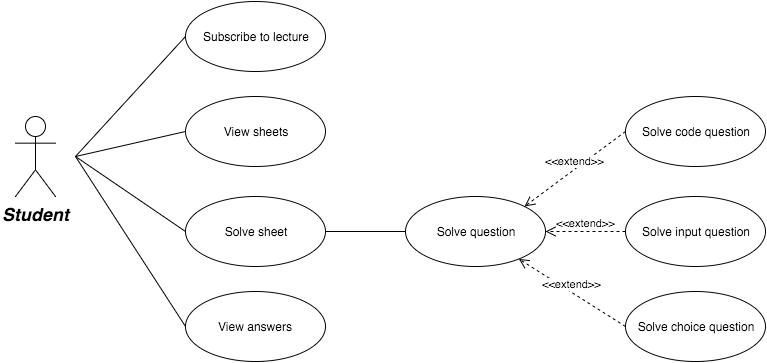
\includegraphics[width=\textwidth,height=\textheight,keepaspectratio]{cases}
	\caption{Use cases for students}
\end{figure}

\begin{figure}[H]
  \centering

	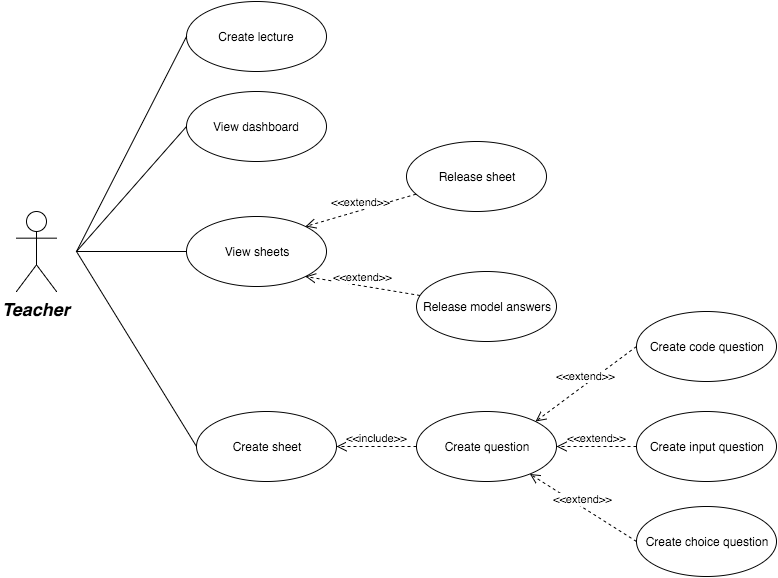
\includegraphics[width=\textwidth,height=\textheight,keepaspectratio]{cases2}
	\caption{Use cases for teachers}
\end{figure}

\subsection{System architecture}
\paragraph{User interface}
Since the user's are assumed to be somewhat technically savvy , the application takes some liberties with having a limited amount of help and information banners since it works similarly to other website the target audience is familiar with.
Overall the application is meant to have a flat design that looks good on any resolution.
Each lecture has a colour chosen by the teacher and shows up throughout the user interface so the user knows which lecture they are looking at.

\subsection{Third party libraries}

\subsubsection{React}
A javascript library that allows the project to have isolated , reusable components that build up all of the user interface

\subsubsection{Chromath} 
A javascript library that can manipulate colours. It is used within the dashboard to compute darker shades of the lecture color - this is useful for both the charts ( each section of the chart is a different colour ) and for the transition matrix ( the higher the transition count , the darker the shade ).

	It is statically included in the project.
	
\subsubsection{CodeMirror}
A javascript library that provides an embeddable code editor. Used to let user's write their own code.

\subsubsection{Markdown-it}
A javascript library used to render Markdown , in both the title preview on the sheet creation page and the actual sheet that the user sees.

\subsubsection{Highlight}
A javascript library to highlight code syntax , used internally by Markdown-it
	
\subsubsection{JQCloud}
A javascript library used to render a word cloud in the dashboard for input questions.

\subsubsection{Levenshtein-ffi}
A ruby gem that allows fast calculation of Levenshtein distances for answer's in the input question's dashboard.

\subsubsection{pg}
A ruby gem for Postgres support

\subsubsection{Devise}
A ruby gem that simplifies authentication

\subsubsection{ReactRails}
Support for React in Rails applications

\subsubsection{Typescript Rails}
Automatic compilation of typescript files as part of the rails asset pipeline.


\chapter{Implementation}

\section{Languages and Frameworks}
\subsection{Front end} 
Since the front end of the project is a web app , HTML and CSS were used to create the user interface. However for the programming Typescript was used instead of Javascript.

\paragraph{Typescript} is a super set of Javascript , made by Microsoft. It adds useful language features to Javascript such as a type system , generics , classes and more. The addition of these features helps the code base be more readable and more maintainable.

In particular having types allows the code to be more easily refactored and reduces redundant documentation (such as including type information in comments).

It is compiled to Javascript before being served to the user and all the functionality is compile-time only so there is no performance penalty in using it.

\paragraph{User interface}
The fronted of the application is mostly tailored , in other words the UI components are made specifically for this project. One of the reasons for this is because lecture colour is an important visual cue in the application's visual design and colouring the components of existing platforms such as Bootstrap can be glitchy as they were not meant to be used in such a way.

\paragraph{ReactJS} was used to create the UI components. React is a light javascript library used to create reusable components in a functional way. Using it has helped create powerful , contained reusable components that can be customised externally without needing to dig into their implementation ( which can be useful for future development ) . They also allow for simple colouring by passing around the lecture colour when creating a component.

\subsection{Backend} 
The main backend written in Ruby , using the Ruby on Rails web framework. The main reason for choosing this framework was that it is proven to be reliable and has a very healthy developer ecosystem. Thus there are a lot of up to date libraries ( or 'gems' ) available to extend the core functionality. In particular , the Typescript gem works seamlessly as part of the Rails asset pipeline to convert the typescript files to javascript.

Another backend was written for handling the execution of user code inside docker contains. This was done using Python and Flask , a python web micro framework. A micro framework was used instead of rails because this part of the system does not involve any advanced features found in full web frameworks ( authentication , models , migration for example )

On the same server as the python backend , Docker is used to create instances where the user code can run safely.

\section{Development Tools}
The backend was developed using RubyMine and PyCharm.
The front-end was written using Visual Studio Code , mainly because it was the only editor at the type that supported TSX files ( Typescript + React inline ).


\section{Rails backend analysis}
This section will explain the structure of code within the backend responsible for the main functionality.

\subsection{Controllers}
Controllers are split by page that the user sees , as well as an additional ApiController which is engineered to be decoupled from the HTML such that it could power a potential mobile or native client.

\paragraph{Application Controller}  Has an action \textit{index} that renders the index page
\paragraph{Lecture Creator Controller} Has an action \textit{index} that renders the page where the teacher can create a lecture
\paragraph{Lecture List Controller} Has an action \textit{index} that renders the page where all the lectures the user created and subscribed to are listed , as well as a \textit{subscribe} method that handles rendering the subscriptions page
\paragraph{Sheet Creator Controller} Has an action \textit{index} that renders the page where the teacher can create sheets
\paragraph{Sheet Dashboard Controller} Has an action \textit{index} that renders the dashboard page that the teacher sees
\paragraph{Sheet Editor Controller} Has an action \textit{index} that renders the sheet editing page where the student can answer a sheet. It also contains an action \textit{update\textunderscore sheet}  that handles updating the user's answer
\paragraph{Sheet Manager Controller} Has an action \textit{index} that renders the page where the teacher can manage all the sheets of his lecture
\paragraph{API Controller} Contains the following methods:
\begin{itemize}
	\item \textit{\textbf{subscribe}} Subscribes the current user to a lecture with id \textit{lecture \textunderscore id}
	\item \textit{\textbf{statistics\textunderscore for \textunderscore question}} Collates and returns the statistics for a given question
	\item \textit{\textbf{completions}} Returns the answers who correctly solved a question
	
	\item \textit{\textbf{lectures}} Returns an object with two properties , \textit{subscribed} which contains the lectures the user is subscribed to and \textit{created} which the user created (is a teacher of)
	\item \textit{\textbf{lecture}} Returns a single lecture information given an id
	\item \textit{\textbf{full \textunderscore sheet}} Returns information about a sheet. Object returned contains the following field : \textit{lecture , sheet , questions , answers , modelAnswers } and \textit{percentage}
	\item \textit{\textbf{sheets}} Returns a list of sheets
	\item \textit{\textbf{create  \textunderscore  sheet}} Creates a sheet given a sheet and an object which represents the new sheet. It will return any errors if any
	\item \textit{\textbf{update \textunderscore sheet}} Updates the name , live status or result status of a given sheet
	\item \textit{\textbf{create \textunderscore lecture}} Creates a lecture with a given name and colour
	\item \textit{\textbf{delete \textunderscore sheet}} Deletes a given sheet
	\item \textit{\textbf{delete \textunderscore lecture}} Deletes a given lecture
	\item \textit{\textbf{lecture \textunderscore users  \textunderscore  count}} Return the number of users subscribed to a lecture
	\item \textit{\textbf{update \textunderscore lecture}} Updates the name or colour of a lecture
	\item \textit{\textbf{stats}} Collates statistics and any metadata computed from them (such as transition matrices)
	\item \textit{\textbf{search}} Searches for a keyword and returns all sheets and lectures that contain it
	\item \textit{\textbf{user \textunderscore info}} Return the email of the logged in user
\end{itemize}

\section{Front end analysis}
The front end is mostly composed of React components; React uses a special file type called JSX which allows the mixing of javascript and HTML in the same file. JSX files go though a compilation phase to become plain JS files.

In this project , Typescript is used instead of javascript , so the files written in the project are TSX files , which compile down to JSX and then to JS.

\subsection{React components}
\paragraph{LectureCreatorPage} The state contains a \textit{\textbf{name}} and \textit{\textbf{color}} which are selected by the user and send using POST when the user presses create lecture.
\paragraph{LectureItem} The component takes a lecture object and renders a single Lecture box
\paragraph{LecturePage} Takes two arrays of lecture objects , one for lectures created and one for subscribed lectures , then renders two sets of LectureItem
\paragraph{SubscribePage} Takes a single lecture object and prompts the user to subscribe to it
\paragraph{SheetCreatorPage} Takes a single lecture object ; this page let's the user create a sheet. It has the following state:
\begin{itemize}
	\item \textit{\textbf{items}} An array of questions that the user is creating for this sheet
	\item \textit{\textbf{name}} The name of the sheet
	\item \textit{\textbf{description}} The description of a sheet
	\item \textit{\textbf{errors}} A map , where the key is a number representing the question index and the value is a list of errors for that question
	\item \textit{\textbf{dragging}} Whether the user is dragging an element to create a new question
\end{itemize}
\paragraph{InputCreator} A component for creating an input question. Takes the following parameters:
\begin{itemize}
	\item \textit{\textbf{color}} The color of the lecture
	\item \textit{\textbf{question}} The question this element is editing/representing
	\item \textit{\textbf{key}} Used internally by React
	\item \textit{\textbf{onDelete}} A function called when the question is deleted
	\item \textit{\textbf{errors}} A list of strings , representing errors with this question
\end{itemize}
\paragraph{CodeIO} An object with an input field and output field (both strings)
\paragraph{CodeCreatorIO} A component with an input textbox and an output textbox. Used to represent a test case in the code question. It takes a CodeIO object which contains a Input and Output field , changes are reflected inside this object
\paragraph{CodeCreator} A component for creating a code question. It allows the user to choose the language and create tests which are instances of CodeIO and are represented by CodeCreatorIO. It has the following properties:
\begin{itemize}
	\item \textit{\textbf{color}} The color of the lecture
	\item \textit{\textbf{question}} The code question this component represents
	\item \textit{\textbf{index}} The index of the question
	\item \textit{\textbf{onDelete}} A function called when the question is deleted
	\item \textit{\textbf{errors}} A list of strings , representing errors with this question
\end{itemize}
\paragraph{ChoiceCreatorAnswer} A component that represents an answer for a choice question. Takes an answer object , the lecture color and a onDelete handler.
\paragraph{ChoiceCreator} A component for creating a choice question. It allows the user to create choices for the user to select.. Takes the following parameters:
\begin{itemize}
	\item \textit{\textbf{color}} The color of the lecture
	\item \textit{\textbf{question}} The question this element is editing/representing
	\item \textit{\textbf{key}} Used internally by React
	\item \textit{\textbf{onDelete}} A function called when the question is deleted
	\item \textit{\textbf{errors}} A list of strings , representing errors with this question
\end{itemize}
\paragraph{SheetDashboardPage} The page where the teacher can see the stats of a sheet. Takes a lecture and a list of questions.
\paragraph{InputStats , CodeStats , ChoiceStats} Components that shows the statistics for the specific type of question. Takes a question and the lecture color.
\paragraph{ActivityIndicator} A component that shows a pie chart that represents the user's who have completed a question succesfully. Takes the following parameters:
\begin{itemize}
	\item \textit{\textbf{question}} The question
	\item \textit{\textbf{color}} The color of the lecture
	\item \textit{\textbf{percentage}} The percentage of students who solved the question
	\item \textit{\textbf{correct}} The number of students who solved the question
	\item \textit{\textbf{wrong}} The number of students who did not solve the question
\end{itemize}
\paragraph{SheetEditPage} The page where the student can complete the sheet. Takes the following properties:
\begin{itemize}
	\item \textit{\textbf{questions}} A list of questions in the sheet
	\item \textit{\textbf{shet}} The sheet the user is answering
	\item \textit{\textbf{lecture}} The lecture the sheet belongs to
	\item \textit{\textbf{answers}} The user's answers
	\item \textit{\textbf{modelAnswers}} The model answers for this sheet
	\item \textit{\textbf{percentage}} The percentage of questions that the user solved
\end{itemize}
\paragraph{InputQuestion , CodeQuestion , ChoiceQuestion} Components that show the questions to the user and let them answer it. Each takes a question , an answer , a color , a model answer and a boolean that represents whether the sheet has model answers released.
\paragraph{SheetManagerPage} The page where the teacher can manage the sheets in the lecture.
\paragraph{SheetControl} A component that represents a sheet and let's the teacher release the model answers , delete it or access the dashboard
\paragraph{SheetsPage} The student view of all the sheets , takes a lecture.
\paragraph{SheetItem} A component that represents a sheet that the student can access. Takes a sheet object.

There are also some shared components:

\paragraph{CheckBox} A checkbox , takes a boolean that represents whether it's checked , a color and a onChange handler.
\paragraph{ColorPicker} Let's the user pick select a color. Takes a onPicked handler that is triggered when a color is selected.
\paragraph{Header} A component that sits at the top of the pages , used for navigation. Takes the following properties:
\begin{itemize}
	\item \textit{\textbf{title}} The title of the page , shown on the left
	\item \textit{\textbf{name}} The name of the user logged in
	\item \textit{\textbf{color}} The color of the lecture
	\item \textit{\textbf{onBack}} Handler , triggered when back button is clicked
	\item \textit{\textbf{foreground}} The foreground color of the header
	\item \textit{\textbf{hideBack}} Whether the back button should be shown.
\end{itemize}
It also has the following state:
\begin{itemize}
	\item \textit{\textbf{showMenu}} Whether the user menu should be shown
	\item \textit{\textbf{showSearch}} Whether to show the search panel
	\item \textit{\textbf{searchSheets}} The sheets found by searching
	\item \textit{\textbf{searchLectures}} The lectures found by searching
	\item \textit{\textbf{query}} The search query typed in the search box
\end{itemize}
\paragraph{IDFactory} Used to generate new IDs for React keys
\paragraph{LCButton} A reusable colourable button , takes a piece of text for the content , a color , an onClick function and a style object.
\paragraph{MDPreview} A reusable component for previewing Markdown. Takes a piece of markdown code and renders it.
\paragraph{SearchDropdown} Used to show search results. Takes the following parameters:
\begin{itemize}
	\item \textit{\textbf{shouldShow}} Whether the search panel should be visible
	\item \textit{\textbf{sheets}} The sheets found by search
	\item \textit{\textbf{lectures}} The lectures found by search
	\item \textit{\textbf{color}} The color of the lecture
	\item \textit{\textbf{query}} The text entered in the search bar
\end{itemize}
\paragraph{SegmentedButton} A segmented button control that let's the user select between options. Takes the following parameters:
\begin{itemize}
	\item \textit{\textbf{color}} The color of the lecture
	\item \textit{\textbf{labels}} An array of strings representing the choices the control provides
	\item \textit{\textbf{style}} Additional styling provided externally
	\item \textit{\textbf{onSelected}} A function triggered when the selection changes
	\item \textit{\textbf{selectedIndex}} The currently selected item
	\item \textit{\textbf{itemPadding}} The padding of each item in the control
\end{itemize}
\paragraph{TextArea} A stylised text area
\paragraph{TextBox} A stylised text box

\textcolor{red}{//example code here and in the typescript}
\textcolor{red}{append styles to React}

\section{Unit testing}
Unit testing was used to make sure changes and additions to the system did not break or alter any previous functionality.

Purpose:
\begin{enumerate}
	\item To make sure existing functionality was not compromised
	\item To ensure that the database settings worked as intended ( defaults , uniqueness etc)
	\item Components of the system all complied with security , such as preventing user's from editing other people's date or gaining access to data they are not allowed to see
\end{enumerate}




\section{Third party libraries} \label{libs}

\subsection{React}
A javascript library that allows the project to have isolated , reusable components that build up all of the user interface

\subsection{Chromath} 
A javascript library that can manipulate colours. It is used within the dashboard to compute darker shades of the lecture color - this is useful for both the charts ( each section of the chart is a different colour ) and for the transition matrix ( the higher the transition count , the darker the shade ).

	It is statically included in the project.
	
\subsection{CodeMirror}
A javascript library that provides an embeddable code editor. Used to let user's write their own code.

\subsection{Markdown-it}
A javascript library used to render Markdown , in both the title preview on the sheet creation page and the actual sheet that the user sees.

\subsection{Highlight}
A javascript library to highlight code syntax , used internally by Markdown-it
	
\subsection{JQCloud}
A javascript library used to render a word cloud in the dashboard for input questions.

\subsection{Levenshtein-ffi}
A ruby gem that allows fast calculation of Levenshtein distances for answer's in the input question's dashboard.

\subsection{pg}
A ruby gem for Postgres support

\subsection{Devise}
A ruby gem that simplifies authentication

\subsection{ReactRails}
Support for React in Rails applications

\subsection{Typescript Rails}
Automatic compilation of typescript files as part of the rails asset pipeline.


\chapter{Professional and Ethical Issues}
Either in a seperate section or throughout the report demonstrate that you are aware of the \textbf{Code of Conduct \& Code of Good Practice} issued by the British Computer Society and have applied their principles, where appropriate, as you carried out your project.

\section{Section Heading}

\chapter{Results/Evaluation}

In this section we will explore whether the project has met the requirements that were set in the requirements section of this report as well as other general aspects of the software that can be evaluated.

One of the core requirements was to let the teacher create different types of question and collate them into a sheet. Since this was a core mechanic of the system , it was one of the first things to be implemented. The teacher can create choice questions (student selects one of multiple choices) , input questions (students can write any text into a text box) and code questions (students can write their own code to solve a question. Furthermore the platform was built with this requirement in mind such that it can be extended later.

Markdown is used to write the body of the questions , this allows the teacher to include rich formatting within the question text. This useful because it can make questions more expressive and easier for the user to understand.


Teachers can easily create a lecture and invite students to subscribe to it by sharing a link. After they are subscribed they can access all the sheets that the teacher has chosen to go live. As student complete the sheet , the teacher can monitor the results so that they may know how to proceed further with the lecture. 
When the teacher decides the sheet time is over , he may release the model answers so the user can see their score and what the correct answer is. If the student accesses a sheet after the model answers are released , they will not be able to submit any changes , but may review their answers.

Docker and container technology allow the system to run student code in a safe way. That coupled with the fact that the languages do not have pointer arithmetic / unsafe operations and run in a non root mode ensures the risk of malicious attack using the student code as a vector is minimised if not completely avoided.

The front end has a shared folder which contains components that can be reused across different pages ; they are generic components but can be customised without the need to modify their implementation.

Another requirement was the extensibility of the platform ; the code and database schema are made in such a way that adding more question types and their respective view in the dashboard is trivial. By using JSON for the core definitions of the questions and answers allows the platform to be well positioned for further development.

Anonymity is an important part of this platform , in fact the only identifiable information asked of the user is their email address. Furthermore data is partitioned such that a user may not get access to data they are not supposed to see , they may also not update or attempt to modify or create a resource that belongs to a resource they do not have permission to interact with.

\subsection{Limitations}
There were some things that were simplified or postponed for the sake of keeping in line with deadlines and achieving all the compulsory requirements that I have set. Thus the system does have some limitation (solutions to those limitations will be explored in the next section)

\begin{itemize}
	\item Code question can be either Java or Python based. This is a limitation imposed to decrease the surface area for bugs that would arise from allowing more languages.
	\item Sheets cannot be edited after they are created. This is because changing the questions as the sheet is live could invalidate existing statistical data retrieved from users completing the question.
	\item Teacher cannot kick out or manage users. This is because currently the system aims to anonymise users so they may not feel discouraged from completing the questions
	\item The website is glitchy and may not work at all on some mobile devices. This is especially true for pages where the user may enter a core
\end{itemize}

\subsection{Security}
While the system is not meant to contain any sensitive data , it is important that the users of the system can be assured that their data is private. 
There are safeguards in place to ensure that a malicious agent may not successfully acquire information they are not entitled to , this functionality is unit tested to ensure it stays this way across releases of the software.
Another layer of security is in the system that executes the student's arbitrary code.
The code runs in a docker container and can only run within either the java virtual machine or the python interpreter. Not allowing low level code to run discourages any traditional security holes such as buffer overflows.
Furthermore , even if someone manages to execute code such that they break out of the language runtime and the docker container - the containers run on a server separate from the main server. Thus they cannot access the database or compromise the system.

\subsection{Overall}
The main purpose of the system was to provide teacher's a way to handle handing out sheets digitally and analyse the result easily in real time. It was built in such a way that not only fulfilled this requirement but also provides a platform that is easily extendable such that more question types can be added without having to modify the existing infrastructure.

\chapter{Conclusion}

\section{Thoughts on project}
This project has taught me a number of things , the most important of which I believe to be making decisions about how time is allocated.
When this project began , my main focus was data aggregation and I had planned to do a lot of work regarding engaging the user in novel ways to try to gauge their under understanding of a subject. However it became apparent to me ( after being advised by my supervisor) that data visualisation and extracting information from the aggregated data is equally important and in fact , the data is not of much use in an unrefined form.
Another thing I learned was the importance of proper mocking up and feature freezes as I have rewritten several components of the system multiple times during the course of the project. This was especially time consuming as I have written most of the UI elements from scratch.

I firmly believe that this project has fulfilled its purpose - which is to create a platform for teacher to user interaction. Both the underlying framework and the user interface have been prepared in such a way that they can extended very easily with more question types and more visualisation options.


\section{Future work}
There are a number of ways to improve the project , the system is implemented in such a way that adding more functionality can be done seamlessly without breaking or having to alter any major components of the system.

Ideas for improvements:
\begin{itemize}
	\item More question types. For example questions that revolve around web development ( such as asking the user to create a html/css layout from an image) or unix command line tools ( asking the user to complete some command line workflow ). This should be easy to implement as the database schema for questions is very flexible and does not make any assumptions about the type of data a question expresses
	\item Better user management for the teacher , allowing them to kick , filter and analyse student progress. This would involve adding a lot more UI components and possibly other pages
	\item Allowing teacher to edit the title/body of questions after the sheet is created. Easy to implement the technical aspect of it , however it would not fit within any current place in the UI and would require an additional page
	\item Password enabled lectures , or alternatively geo-locked lectures. Fairly simple to implement but needs to have extra logic in place to deal with changing the password and so on
	\item Mobile apps for Android and iOS to expand the pool of students who have a device that can use the project. Takes time but overall the backend would not have to be changed much as it already exposes most functionality via a simple REST API
\end{itemize}


%%%%%%%%%%%%%%%%%%%%%%%%%%%%%%%%%
% References
%%%%%%%%%%%%%%%%%%%%%%%%%%%%%%%%%
\bibliographystyle{plain}
\bibliography{references}
\addcontentsline{toc}{section}{Bibliography}

%%%%%%%%%%%%%%%%%%%%%%%%%%%%%%%%%
% Appendices
%%%%%%%%%%%%%%%%%%%%%%%%%%%%%%%%%
\appendix
\include{Appendices/appendix}
\chapter{User Guide}
\section{Instructions}
You must provide an adequate user guide for your software. The guide should provide easily understood instructions on how to use your software. A particularly useful approach is to treat the user guide as a walk-through of a typical session, or set of sessions, which collectively display all of the features of your package. Technical details of how the package works are rarely required. Keep the guide concise and simple. The extensive use of diagrams, illustrating the package in action, can often be particularly helpful. The user guide is sometimes included as a chapter in the main body of the report, but is often better included in an appendix to the main report.

\chapter{Source Code}
\section{Instructions}
Complete source code listings must be submitted as an appendix to the report. The project source codes are usually spread out over several files/units. You should try to help the reader to navigate through your source code by providing a ``table of contents'' (titles of these files/units and one line descriptions). The first page of the program listings folder must contain the following statement certifying the work as your own: ``I verify that I am the sole author of the programs contained in this folder, except where explicitly stated to the contrary''. Your (typed) signature and the date should follow this statement.

All work on programs must stop once the code is submitted to KEATS. You are required to keep safely several copies of this version of the program and you must use one of these copies in the project examination. Your examiners may ask to see the last-modified dates of your program files, and may ask you to demonstrate that the program files you use in the project examination are identical to the program files you have uploaded to KEATS. Any attempt to demonstrate code that is not included in your submitted source listings is an attempt to cheat; any such attempt will be reported to the KCL Misconduct Committee.

\textbf{You may find it easier to firstly generate a PDF of your source code using a text editor and then merge it to the end of your report. There are many free tools available that allow you to merge PDF files.}


\end{document}
